% Préambule APMEP - Annales
% Auteurs
% tapuscrit : Mathieu Drillet
% relecture : François Kriegk
% figures TikZ :
% figures pstricks :
% modifications :
% Remerciements :
% version 1 : 2026-06-30
\documentclass[12pt,a4paper,french]{article}

% Packages
%%% codage et police utilisée
\usepackage[T1]{fontenc}
\RequirePackage{iftex}
\iftutex % moteur utf-8 lualatex, xelatex
\usepackage{fourier-otf} % remplace fourier pour moteur utf8 (LuaLaTeX, XeLaTeX)
% Alternatives nécéssite (LuaLaTeX, XeLaTeX)
\usepackage{hyperref}
%\usepackage{fontspec}% pour utiliser des fontes système
\else % pour les autres moteurs latex, pdflatex
\usepackage[utf8]{inputenc}
\usepackage{fourier}
\usepackage{amsmath,amssymb}
\usepackage[dvips]{hyperref}
\renewcommand{\ttdefault}{lmtt}
\fi
\usepackage[normalem]{ulem}
\usepackage{pifont}
\usepackage{lscape}
% tableaux
\usepackage{multicol}
\usepackage{multirow}
\usepackage{tabularx}
\usepackage{tabularray}
% texte et composition
\usepackage{textcomp}
\usepackage{babel}
\usepackage[np]{numprint}
%
\usepackage{fancyhdr}
\usepackage{makeidx}
\makeindex
% pour le symbole €
\usepackage{eurosym}
\DeclareRobustCommand{\officialeuro}{%
	\ifmmode\expandafter\text\fi
	{\fontencoding{U}\fontfamily{eurosym}\selectfont e}}
\AtBeginDocument{\renewcommand{\euro}{\officialeuro}}
% couleurs étendues
\usepackage{xcolor}
% pour les listes
\usepackage{enumitem}
% Enumérations réglage par défaut
\setlist[itemize]{label=\textbullet,leftmargin=5mm,labelwidth=3mm,labelsep=2mm,align=left}
\setlist[enumerate]{labelindent=0pt, leftmargin=5mm, labelsep=2mm, labelwidth=3mm,labelsep=2mm, align= left}
\setlist[enumerate,1]{label = \textbf{\arabic*.}}
\setlist[enumerate,2]{label = \textbf{\alph*.}}
\setlist[enumerate,3]{label = \textbf{\roman*.}}
% pour l'ajustement des boites (figures…)
\usepackage{adjustbox}
% pour ne pas commencer un exercice en fin de page
\usepackage{needspace}
%
% Taille de la zone d'écriture
\usepackage[left=1.5cm,right=1.5cm,top=3cm,bottom=3cm]{geometry}
\setlength{\headheight}{15pt}
\setlength{\parindent}{0mm}
%
% Formatage du pdf
\hypersetup{%
	pdfauthor = {APMEP},
	pdfsubject = {Troisième, Série générale},
	pdftitle = {Brevet des collèges    -- Session 2026},
	allbordercolors = white,
	pdfstartview=FitH
}
% Pour scratch (code)
\usepackage{scratch3}
% Pour le code Python
\usepackage{listings}
\lstdefinestyle{python}{
	language=Python,
	basicstyle=\ttfamily\small,
	keywordstyle=\color{blue}\bfseries,
	commentstyle=\color{gray}\itshape,
	stringstyle=\color{orange},
	numbers=left,
	numberstyle=\tiny\color{gray},
	breaklines=true,
	frame=single,
	backgroundcolor=\color{gray!5},
	tabsize=4
}
% usage (exemple)
%\begin{lstlisting}[style=python]
%def seuil():
%    n = 1
%    p = 0.5
%    while p < 0.6 :
%       n = n + 1
%       p = p*7/15 + 1/3
%    return n
%\end{lstlisting}


% Pour une visualisation de type tableur
\usepackage{pas-tableur}
%
%% pour PsTricks
\usepackage{pst-bezier}%% AVANT les autres PST
\usepackage{pstricks-add}
\usepackage{pst-func,pst-tree,pst-circ}
\usepackage{pst-eucl}
%% pour TikZ
\usepackage{tikz,pgfplots,pgf,tkz-tab,tikzpagenodes}
\usetikzlibrary{calc,patterns,decorations,arrows.meta,patterns.meta,arrows}
\pgfplotsset{compat=1.18,/pgf/number format/.cd,use comma}
\usepackage{icomma} % gestion des espaces autour des virgules
\DeclareMathSymbol{;}{\mathbin}{operators}{"3B}% pour un espacement correct du ; en mode maths
%%%%%%%%%%%%%%%%%%%%%%%%%%%%%%%%%%%%%%%%%%
% Définitions
%
% notation en mode mathématique et hors mode mathématique
\newcommand{\R}{\ensuremath{\mathbb{R}}}
\newcommand{\N}{\ensuremath{\mathbb{N}}}
\newcommand{\D}{\ensuremath{\mathbb{D}}}
\newcommand{\Z}{\ensuremath{\mathbb{Z}}}
\newcommand{\Q}{\ensuremath{\mathbb{Q}}}
\newcommand{\C}{\ensuremath{\mathbb{C}}}
%
\providecommand{\up}{\textsuperscript}
%
\newcommand{\vect}[1]{\overrightarrow{\,\mathstrut#1\,}}
\newcommand{\vectt}[1]{\overrightarrow{\,\mathstrut\text{#1}\,}}
%
\def\Oij{$\left(\text{O};\vect{\imath},\vect{\jmath}\right)$}
\def\Oijk{$\left(\text{O};\vect{\imath},\vect{\jmath},\vect{k}\right)$}
\def\Ouv{$\left(\text{O};\vect{u},\vect{v}\right)$}
%
\newcommand{\ds}{\displaystyle}
%
\renewcommand{\d}{\mathrm{\,d}}
\renewcommand{\i}{\mathrm{\,i\,}}
\newcommand{\e}{\mathrm{\,e\,}}
%%%%%%%%%%%%%%%%%%%%%%%%%%%%%%%%%%%%%%%%%%%


\begin{document}

	%---------------------------------------------------------
	% Réglage entête, pied de page
	%---------------------------------------------------------
	\rhead{\textbf{A. P{}. M. E. P{}.}}
	\lhead{\small Corrigé}
	\lfoot{\small{Asie}}
	\rfoot{\small{15 juin 2026}}
	\pagestyle{fancy}

	\thispagestyle{empty}


	%---------------------------------------------------------
	% Titre
	%---------------------------------------------------------
	\begin{center}
		{\Large \textbf{\decofourleft~ Brevet des collèges ~\decofourright\\[10pt]Corrigé\\[10pt]  Série générale -- Asie -- 15 juin 2026 }}
	\end{center}

	\marginpar{\rotatebox{90}{\textbf{A. P{}. M. E. P{}.}}}


\section*{Partie 1 -- Automatismes -– 6 points}

	\subsection*{Question 1}
		$\np{45310}=\np{4,5310}\times \np{10000}=\np{4,531}\times 10^4$.

		\textbf{Réponse B}.

	\subsection*{Question 2}
		Dans l'expression \quad $(4x – 3)(4x + 3)$,

		on reconnaît le premier membre de l'identité remarquable \quad $(a+b)(a-b)=a^2-b^2$.

		En identifiant $a=4x$ et $b=3$, on obtient : \quad $(4x)^2-3^2=16x^2-9$.

		\textbf{Réponse C}.

	\subsection*{Question 3}
		Le volume d'un pavé droit est le produit de sa longueur par sa largeur par sa hauteur.

		On a donc :\quad $\mathcal{V}=4,5\times 4\times 10={180}$(cm$^3$).

		\textbf{Réponse A}.

	\subsection*{Question 4}
		Le critère de divisibilité par 9, c'est de voir si la somme des chiffres du nombre est divisible par 9.

		$2+0+2+5=9 = 9 \times 1$ \quad donc $\np{2025}$ est divisible par 9.

		$2+0+2+6=10 $\quad donc \quad $\np{2026}$ n'est pas divisible par 9.

		Donc \textbf{Réponse B}.

	\subsection*{Question 5}
		Effectuons la conversion :
		\quad
		$\begin{aligned}[t]
		\np[km]{9}  &\to  \np[min]{45} &\text{ en divisant par 3}\\
		\np[km]{3}  &\to  \np[min]{15} & \text{ en multipliant par 4}\\
		\np[km]{12} &\to  \np[min]{60} & \\
		\end{aligned}$

		Et \np[min]{60}, c'est une heure, donc sa vitesse est de 12 km/h.

	\subsection*{Question 6}
		Comme les secteurs sont de taille égale, on est en situation d'équiprobabilité, la probabilité est donc obtenue en divisant le nombre d'issues favorables par le nombre d'issues total.

		Il y a 2 casques audio sur 10 secteurs, donc la probabilité est de $\dfrac{2}{10}$, c'est-à-dire, après simplification $\dfrac{1}{5}$.

	\subsection*{Question 7}

		\emph{Méthode 1 :}

		$60\times \dfrac{10}{100}=6$, \quad 10\,\% de 60\,\euro{} représentent donc 6\,\euro{}.

		$60-6=54$, \quad son nouveau prix après une baisse de 10\,\% est de 54 \euro{}.

		\emph{Méthode 2 :}

		Baisser de 10\,\%, c'est multiplier par : \quad $c = 1 - \dfrac{10}{100} = 0,9$.

		$60c = 60 \times 0,9 = 6 \times 9 = 54$,\quad son nouveau prix après une baisse de 10\,\% est de 54 \euro{}.

	\subsection*{Question 8}
		La somme des angles dans un triangle vaut 180\textdegree.

		$180 = 90+ 40 + x$\quad soit \quad $x =180 -(90+40)=50$.

		L'angle $\widehat{\mathrm{BAC}}$ a donc une mesure de 50\textdegree.

	\subsection*{Question 9}

\begin{enumerate}[label=\textbf{\alph*.},left=5mm]
\item Le nombre d'élèves ayant participé à ce contrôle est la somme des effectifs des notes :

$3+4+0+4+5+5+0+0+3+0+2+1=27$,\quad il y a 27 élèves.

\item %$28 \div 2 = 14$,\quad la moitié de l'effectif est 14.
La 13\up{e} et la 14\up{e} valeur sont égales à 11 : c'est la médiane.
%L'effectif total est pair, donc la médiane est la moyenne des deux valeurs centrales : la 14\up{e} et la 15\up{e} dans la série ordonnée.
%Dans l'ordre croissant :
%\begin{itemize}
%\item Les trois premières valeurs sont des 7;
%\item les quatre valeurs suivantes, de la 4\up{e} à la 7\up{e}, sont des 8;
%\item les quatre valeurs suivantes, de la 8\up{e} à la 11\up{e} sont des 10;
%\item les cinq valeurs suivantes, de la 12\up{e} à la 16\up{e} sont des 11.
%\end{itemize}
%
%Ainsi, la 14\up{e} et la valeur dans l'ordre croissant sont égales à 11.

%		$\dfrac{11+11}{2}=11$,\quad a médiane est donc 11.
		\end{enumerate}
		\newpage

\section*{Partie 2 -- Raisonnement et résolution de problèmes -- 14 points}

\section*{Exercice 1 (2,5 points)}

\begin{enumerate}
	\item Au bout de 24 mois, le prix payé par Lola est :
	\begin{itemize}
		\item \textbf{Offre A} : \quad $175+16\times 24=559$;
		\item \textbf{Offre B} : \quad $23\times 24=552$
	\end{itemize}

	$552 < 559$, \quad donc l'offre B est plus intéressante au bout de 24 mois.

	\item \begin{enumerate}
		\item Comme $x$ représente le nombre de mois, on doit prendre le tarif par mois et le multiplier par $x$, et puis, on doit ajouter le prix payé à l'achat, éventuellement.

		La fonction $f$ correspond à l'offre \textbf{A} et la fonction $g$ à l'offre \textbf{B}.

		\item Puisque $f(x)$ est le prix payé au bout de $x$ mois avec l'offre A et $g(x)$ celui payé avec l'offre B, pour répondre à la question, on cherche à résoudre l'équation :
		\begin{align*}
		f(x)&=g(x)\\
		175+16x&=23x\\
		16x-23x&=-175\\
		-7x&=-175\\
		x&=\dfrac{-175}{-7}\\
		x&=25
		\end{align*}

		La solution de l'équation est 25.

		Cela signifie qu'au bout de 25 mois, les deux formules donnent le même prix.

		\item $25>24$,\quad donc on n'est plus dans la période d'engagement.
	\end{enumerate}
\end{enumerate}

\newpage
\section*{Exercice 2 (3 points)}

\begin{enumerate}
	\item Le triangle OAD est rectangle en A.

	D'après le théorème de Pythagore, on a :

	$\begin{aligned}
	\mathrm{OD}^2&=\mathrm{AD}^2+\mathrm{AO}^2\\
	8,2^2&=1,8^2+\mathrm{AO}^2\\
	\mathrm{AO}^2&=8,2^2-1,8^2\\
	\mathrm{AO}^2&=64\\
	\mathrm{AO}&=\sqrt{64}& \text{car une longueur est positive.}\\
	\mathrm{AO}&=8.
	\end{aligned}$

	Donc la longueur du segment [AO] est bien de 8 cm.

	\item (BC) et (AD) sont toutes les deux perpendiculaires à la même droite (BO).

	Donc les droites (BC) et (AD) sont donc parallèles.

	\item \begin{itemize}
		\item Les points O, A, B dans cet ordre;
		\item les points O, D, C sont alignés, dans le même ordre;
		\item les droites (BC) et (AD) sont parallèles.
	\end{itemize}

	D'après le théorème de Thalès, on a :\quad $\dfrac{\mathrm{OA}}{\mathrm{OB}}=\dfrac{\mathrm{AD}}{\mathrm{BC}}=\dfrac{\mathrm{AD}}{\mathrm{BC}}$.

	Notamment : \quad $\dfrac{\mathrm{OA}}{\mathrm{OB}}=\dfrac{\mathrm{AD}}{\mathrm{BC}}$.

	En remplaçant par les valeurs connues :\quad $\dfrac{8}{\mathrm{OB}}=\dfrac{1,8}{4,5}$

	Finalement,\quad : $\mathrm{OB}=\dfrac{4,5\times 8}{1,8} =20$.

	Donc la longueur du segment [OB] est 20 cm.

	\item \begin{enumerate}
		\item Le volume du grand cône de hauteur [OB] se calcule ainsi :

		$V_G=\dfrac{\pi \times 4,5^2\times 20}{3}=135\pi\approx \np[cm^3]{424}$.

		\item Calculons le volume du petit cône de hauteur [AO] :

		$V_p=\dfrac{\pi \times 1,8^2\times 8}{3}=\dfrac{216\pi}{25}\approx \np[cm^3]{27}$

		Le volume du gobelet est donc :

		$V_G-V_p\approx 424-21=\np[cm^3]{397}$.
	\end{enumerate}
\end{enumerate}

\newpage
\section*{Exercice 3 (4 points)}

\begin{enumerate}
	\item \begin{itemize}
		\item On choisit 5;

		\item d'une part, le carré de 5 est :\quad $5^2 = 25$;

		puis, en multipliant ceci par 3 :\quad $3 \times 25 = 75$;

		\item d'autre part, en multipliant 5 par 7 :\quad $5\times 7 = 35$;

		\item on additionne les deux nombres :\quad $75+35=110$;

		\item Finalement, on soustrait 6 :\quad $110-6=104$.
	\end{itemize}
	Le \textbf{programme A}, appliqué à 5, donne donc 104.

	\item On veut dans \textsf{B2} le résultat du \textbf{programme A}, appliqué au nombre qui est dans la cellule \textsf{A2} :
	\begin{itemize}
		\item On choisit \textsf{A2};

		\item d'une part, le carré de \textsf{A2} est \textsf{A2} multiplié par lui même:\quad \textsf{A2*A2};

		puis, en multipliant ceci par 3 :\quad \textsf{3*A2*A2};

		\item d'autre part, en multipliant \textsf{A2} par 7 :\quad $7*\textsf{A2}$;

		\item on additionne les deux nombres :\quad \textsf{3 * A2 * A2 + 7 * A2};

		\item Finalement, on soustrait 6 :\quad \textsf{3 * A2 * A2 + 7 * A2 - 6};
	\end{itemize}
	Le \textbf{programme A} sera appliqué par la formule :\textsf{3 * A2 * A2 + 7 * A2 - 6}.

	\item À l'aide du tableur, on constate que lorsqu'on prend $-3$ comme nombre de départ (cellule \textsf{A3}), on obtient 0 (cellule \textsf{B3}).

	\item \begin{itemize}
		\item On choisit $x$;

		\item d'une part, le carré de $x$ est :\quad $x^2$;

		puis, en multipliant ceci par 3 :\quad $3x^2$;

		\item d'autre part, en multipliant $x$ par 7 :\quad $7x$;

		\item on additionne les deux nombres :\quad $3x^2+7x$;

		\item Finalement, on soustrait 6 :\quad $3x^2+7x-6$.
	\end{itemize}

	Avec $x$ comme nombre de départ, une expression littérale du \textbf{programme A} en fonction de $x$ est:\quad $3x^2+7x-6$

	\item \begin{itemize}
		\item On choisit 5;

		\item d'une part, en multipliant 5 par 3 :\quad $3 \times 5 = 15$,

		puis, en soustrayant 2 : \quad $15 - 2 = 13$;

		\item d'autre part, en ajoutant 3 à 5 :\quad $5+3=8$;

		\item on multiplie les deux nombres :\quad $13 \times 8 = 104$;
	\end{itemize}

	En appliquant le \textbf{programme B} à 5, on obtient aussi 104.

	\item \begin{itemize}
		\item On choisit $x$;

		\item d'une part, en multipliant $x$ par 3 :\quad $3x$,

		puis, en soustrayant 2 : \quad $3x-2$;

		\item d'autre part, en ajoutant 3 à $x$ :\quad $x+3$;

		\item on multiplie les deux nombres :\quad $(3x-2)(x+3)$;
	\end{itemize}

	En appliquant le \textbf{programme B} à $x$, on obtient l'expression :\quad $(3x-2)(x+3)$.

	\item Trouvons la forme développée réduite de l'expression littérale du \textbf{programme B} :
	\begin{align*}
	(3x-2)\times (x+3)&=3x\times x+3x\times 3+(-2)\times x+(-2)\times 3\\
	&=3x^2+9x-2x-6\\
	&=3x^2+7x-6
	\end{align*}

	On retrouve la même expression que le \textbf{programme A}, donc Mathis a raison.

	\item Résolvons :
	\begin{center}
	$(3x-2)(x+3) = 0$

	Un produit est nul si et seulement si l'un de ses facteurs est nul ; donc :

	$3x-2=0$ \quad ou \quad $x+3=0$

	$3x=2$\quad ou \quad $x=-3$

	$x=\dfrac{2}{3}$\quad ou \quad $x=-3$
	\end{center}

	Donc l'équation a deux solutions, son ensemble des solutions est :\quad $\mathcal{S}=\left\{-3 ;\dfrac{2}{3} \right\}$.


	Ainsi les valeurs de $x$ pour lesquelles les \textbf{programmes A} et \textbf{B} donnent 0 sont $-3$ et $\dfrac{2}{3}$.
\end{enumerate}


\newpage
\section*{Exercice 4 (2,5 points)}

\begin{enumerate}
	\item FBA est un triangle équilatéral, donc ses trois angles mesurent 60\textdegree{}.

	ABCD est un carré donc ses quatre angles mesurent 90\textdegree{}.

	Les points F, A et E sont alignés, donc $\widehat{\mathrm{FAE}}=180$\textdegree.

	Ainsi\quad $\widehat{\mathrm{EAD}}=180-90-60=30$\textdegree.

	\item Comme il faut 10 pas pour faire un centimètre dans la réalité, il faut 40 pas pour 4 centimètres :
	\begin{itemize}
		\item \textbf{J} représente la longueur en pas du côté du triangle donc \quad $\textbf{J}=40$;

		\item \textbf{M} représente la longueur en pas du côté du carré donc \quad \textbf{M}=40.
	\end{itemize}

	Pour les rotations, il faut comprendre comment les angles se tracent. Imaginons que notre lutin Scratch est \og orienté à 90\textdegree\fg{}, il regarde donc vers la droite.

	Puis, il avance de 40 pas, et il regarde toujours vers la droite.

	On le fait tourner alors pour qu'il regarde dans la direction du prochain segment.

	\begin{center}
	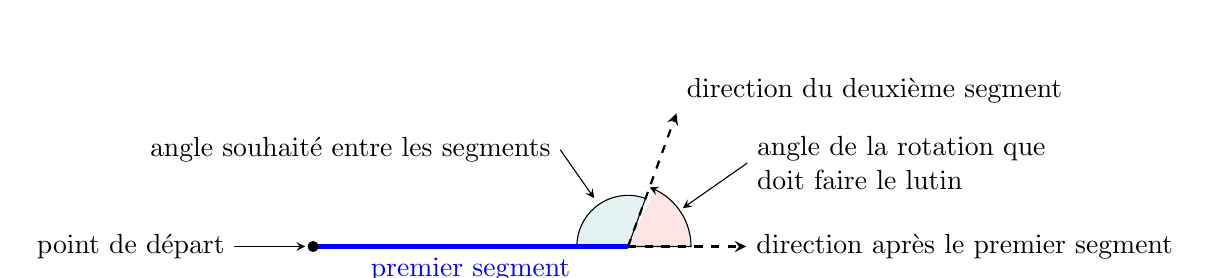
\begin{tikzpicture}[>=stealth]
		\draw[fill=teal!10] (0,0)--(70:0.65) arc (70:180:0.65)--cycle ;
		\draw[<-] (125:0.75)--(125:1.5) node[left]{angle souhaité entre les segments} ;
		\draw[fill=red!10,->] (0,0)--(0:0.8) arc (0:70:0.8) ;
		\draw[<-] (35:0.85)--(35:1.85) node[right,text width=4cm]{angle de la rotation que doit faire le lutin} ;
		\draw[line width=2pt,blue] (-4,0) -- (0,0)node[below,pos=0.5]{premier segment};% -- (70:3)node[right,pos=0.85]{deuxième segment} ;
		\fill (-4,0) circle (2pt);
		\draw[<-] (-4.1,0)--(-5,0)node[left]{point de départ} ;
		\draw[line width=0.8pt,dashed, ->] (0,0) -- (1.5,0) node[right]{direction après le premier segment};
		\draw[line width=0.8pt,dashed, ->] (0,0) -- (70:1.8) node[above right]{direction du deuxième segment};

	\end{tikzpicture}
	\end{center}
	L'angle souhaité entre les segments et l'angle de rotation du lutin Scratch sont donc supplémentaires : leur somme vaut 180\textdegree.

	\begin{itemize}
		\item \textbf{K} représente l'angle de rotation de Scratch, pour un angle souhaité de 60\textdegree{} entre les segments, donc \quad $\textbf{K}=180 -60 = 120$;

		\item \textbf{N} représente l'angle de rotation de Scratch, pour un angle souhaité de 90\textdegree{} entre les segments, donc  \quad $\textbf{N}=180-90= 90$.
	\end{itemize}

	\item Quand le lutin effectue le bloc Triangle, il fait trois rotations de 120\textdegree, et donc il tourne en tout de 360\textdegree{} : il termine la figure en étant revenu à son point de départ (pour fermer le triangle), en ayant la même orientation qu'au début du bloc.

	De même pour le bloc Carré, car il fait quatre rotations de 90\textdegree : là encore, il est revenu à son point de départ (pour fermer le carré) et il a la même orientation qu'au début du bloc.

	L'instruction \begin{scratch}\blockmove{avancer de \ovalnum{50}pas}\end{scratch} après un bloc Triangle ou Carré nous indique qu'on avance de plus de la longueur d'un côté, qui est de 40 pas, il y aura donc une distance de 10 pas entre le point le plus à droite du premier bloc, et le point de départ du bloc suivant. Cela exclut les figures 1, 2 et 4 (dans la figure 4, on a un espace entre les carrés et les triangles qui suivent, mais pas entre les triangles et les carrés qui les suivent) 	.

	Par ailleurs, l'instruction \begin{scratch}\blockmove{tourner \turnleft{} de \ovalnum{30} degrés}\end{scratch} après chaque bloc Triangle ou Carré crée une figure \og circulaire \fg{} (il y aura en tout 6 rotations de 30 degrés, donc à nouveau 360 degrés en tout); cela confirme la \textbf{figure 3}.
\end{enumerate}
\end{document}